\section{Funcionamiento}
\label{sec:funcionamiento}

\begin{table}[!b]
\renewcommand\tabularxcolumn[1]{m{#1}}
\caption{Código de luces del \textit{Chana Monitoring System}}
\label{tab:luces}
\begin{tabularx}{\textwidth}{ccX}
\toprule
\headingc{Color} & \headingc{Estado} & \headingc{Descripción} \\
\topruleb
  \circlefilled{red}    & \textsc{\textbf{apagado}}      & Sin errores. Comprobar \circlefilled{yellow} y \circlefilled{green} para más datos.\\*\midrule
  \circlefilled{red}    & \textsc{\textbf{fijo}}         & El \MIE ha perdido conexión con el \MEE durante demasiado tiempo.\\*\midrule
  \circlefilled{red}    & \textsc{\textbf{intermitente}} & El \MEE ha detectado que el depósito está lleno.\\*\midrule
  \circlefilled{yellow} & \textsc{\textbf{apagado}}      & El \MIE se inició correctamente y se sincronizó con el \ME. Comprobar \circlefilled{red} y \circlefilled{green} para más datos.\\*\midrule
  \circlefilled{yellow} & \textsc{\textbf{fijo}}         & El \MIE está intentando conectar a una red wifi o está en modo gestión.\\*\midrule
  \circlefilled{yellow} & \textsc{\textbf{intermitente}} & El \MIE se ha iniciado correctamente, pero no se ha sincronizado con el \MEE aún.\\*\midrule
  \circlefilled{green}  & \textsc{\textbf{apagado}}      & No hay/ha habido conexión entre el \MIE y el \MEE. Comprobar \circlefilled{red} y \circlefilled{yellow} para más datos.\\*\midrule
  \circlefilled{green}  & \textsc{\textbf{fijo}}         & El \CMS funciona normalmente.\\*\midrule
  \circlefilled{green}  & \textsc{\textbf{intermitente}} & El \CMS funciona normalmente, pero el \MEE tiene la batería baja.\\*\bottomrule
\end{tabularx}
\end{table}

Con el objetivo de maximizar el tiempo de vida de las batería del \MEE, el \MIE es quien proporciona toda la información al usuario del \CMS a través de alarmas sonoras, los testigos \circled{I2}, \circled{I3} e \circled{I4} y la pantalla LCD \circled{I1}. Los testigos y las alarmas sonoras permiten comprobar el estado del \CMS de un vistazo rápido, sin necesidad de comprobar los mensajes que se muestran en la pantalla LCD \circled{I1}. La tabla~\ref{tab:luces} resume los principales estados que representan los diferentes testigos de colores.



En las siguientes subsecciones, se describne en detalle las diferentes informaciones que puede mostrar el \CMS.

\subsection{Arranque}

Cuando el \MIE se conecta a la alimentación USB, éste se enciende de forma automática e intenta conectarse a la red wifi que haya sido configurada a través de la interfaz de gestión (ver sección~\ref{sec:gestion-avanzada}, \textit{\nameref{sec:gestion-avanzada}}). Esto se notifica mediante el testigo de configuración \circled{I3} encendido de forma fija (\circlefilled{yellow}), y mostrando el mensaje \emph{Conectando a red WiFi\ldots} en la pantalla LCD \circled{I1} tal y como muestra la figura \ref{fig:screen-conn-process}.

\begin{figure}[!b]
  \centering
  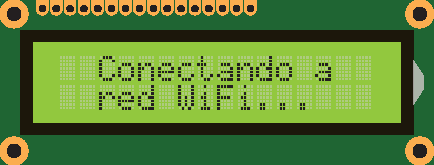
\includegraphics[width=0.6\columnwidth]{images/screen-conn-process}
  \caption{Pantalla del módulo interior -- Conectando a red wifi}
  \label{fig:screen-conn-process}
\end{figure}

\begin{figure}[!b]
  \centering
  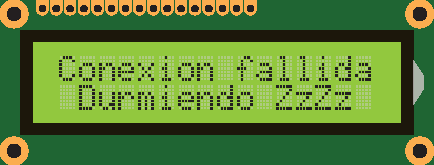
\includegraphics[width=0.6\columnwidth]{images/screen-conn-failed}
  \caption{Pantalla del módulo interior -- fallo de conexión}
  \label{fig:screen-conn-failed}
\end{figure}


En caso de que la conexión falle, el sistema apagará todos los testigos y mostrará el mensaje \emph{Conexion fallida / Durmiendo ZzZz} tal y como muestra la figura~\ref{fig:screen-conn-failed}. El \MI se quedará en ese estado de hibernación hasta que el usuario lo reinicie y compruebe por qué no ha sido posible realizar la conexión (error puntual, cobertura wifi deficiente, \etc).



\subsection{El menú de información}
\label{sec:menu-info}

El menú de información se muestra cuando el \MIE ha arrancado y se ha conectado a una red wifi de forma satisfactoria. Consta de 5 pantallas, que pueden navegarse en la secuencia
~~~\tikz[baseline=-0.63ex,node distance=1em,remember picture]{
\node (n1) {1};
\node (n2) [right=of n1] {2};
\node (n3) [right=of n2] {3};
\node (n4) [right=of n3] {4};
\node (n5) [right=of n4] {5};
\draw[->] (n1) -> (n2);
\draw[->] (n2) -> (n3);
\draw[->] (n3) -> (n4);
\draw[->] (n4) -> (n5);
}
\tikz[remember picture,overlay]{
\draw[->,smooth]  (n5)
to[out=0, in=180]  ($(n5) + ( 0.3cm, 0.00cm)$)
to[out=0, in=0]    ($(n5) + ( 0.3cm,-0.22cm)$)
to[out=180,in=0]   ($(n1) + (-0.3cm,-0.22cm)$)
to[out=180,in=180] ($(n1) + (-0.3cm, 0.00cm)$)
to[out=0, in=180] (n1);
}~~
pulsando el botón multifunción~\circled{I8}.

\textbf{Pasados 60 segundos desde la última pulsación del botón multifunción \circled{I8}, el \MI volverá automáticamente a la pantalla 1.}

\attbegin{Pantallas 1 y 2}
Nada más iniciarse, y mientras el testigo de configuración \circled{I3} se enciende de forma \textbf{intermitente} (\circlefilled{yellow}), sólo se mostrarán las pantallas 3 a 5 hasta que el \MEE realice la primera sincronización de datos y se encienda el testigo de conexión \circled{I4} (\circlefilled{green}).

\textbf{En ese caso, al pasar 60 segundos sin pulsar el botón multifunción \circled{I8}, el \MI volverá automáticamente a la pantalla 3 en lugar de a la pantalla~1.}
\attend

Las pantallas de información que muestre el \MIE en su modo de operación normal son:

\begin{descriptioncompact}

\begin{figure}[!b]
  \centering
  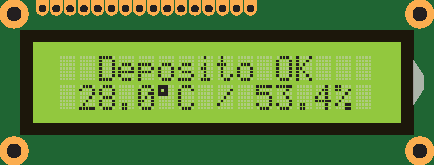
\includegraphics[width=0.6\columnwidth]{images/screen1}
  \caption{Pantalla 1 del módulo interior -- Información exterior}
  \label{fig:screen1}
\end{figure}

\item[Pantalla 1: Información exterior] --- Esta pantalla sólo se muestra cuando el \MEE ha enviado datos de estado recientemente. Como muestra la figura~\ref{fig:screen1}, la primera línea muestra el estado del depósito, mientras que la segunda línea muestra la temperatura y porcentaje de humedad exteriores.

\begin{figure}[t]
\centering
\begin{subfigure}{0.6\columnwidth}
  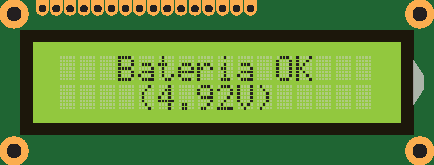
\includegraphics[width=1\columnwidth]{images/screen2a}
  \caption{}
  \label{fig:screen2a}
\end{subfigure}
\\[1em]
\begin{subfigure}{0.6\columnwidth}
  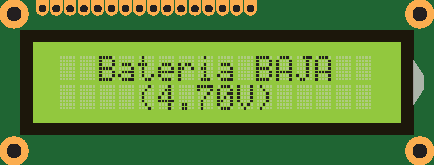
\includegraphics[width=1\columnwidth]{images/screen2b}
  \caption{}
  \label{fig:screen2b}
\end{subfigure}
\caption{Pantalla 2 del módulo interior -- información de batería}
\label{fig:screen2}
\end{figure}

\item[Pantalla 2: información de batería] --- Al igual que la pantalla 1, esta pantalla sólo se muestra cuando el \MEE ha enviado datos de estado recientemente. Como muestra la figura~\ref{fig:screen2}, la primera línea muestra el estado de la batería según el \emph{Umbral de batería baja} (ver sección~\ref{sec:params-interior}, \textit{\nameref{sec:params-interior}}), mientras que la segunda línea muestra el detalle de la tensión proporcionada por las baterías del \MEE. Cuando se muestra el mensaje de \emph{Bateria BAJA}, el testigo de conexión \circled{I4} (\circlefilled{green}) estará encendida de forma intermitente.

\attbegin{Umbral de batería baja}
La temperatura exterior puede afectar al nivel de batería detectado en \mbox{$\pm$0,1 V}. Por tanto, es normal que existan variaciones mínimas en el nivel de batería a lo largo del día. Igualmente, cuando el nivel de batería esté cerca del umbral de batería baja, es normal que el \MIE cambie frecuentemente entre \emph{Batería OK} y \emph{Bateria BAJA} dependiendo de las variaciones de la temperatura exterior.
\attend

\begin{figure}
  \centering
  \includegraphics[width=0.6\columnwidth]{images/screen3}
  \caption{Pantalla 3 del módulo interior -- información de red}
  \label{fig:screen3}
\end{figure}


\item[Pantalla 3: información de red] --- Ésta es la primera pantalla que se muestra cuan\-do el \MIE acaba de iniciarse, el \MEE todavía no ha enviado datos, y el testigo de configuración \circled{I3} (\circlefilled{yellow}) todavía se enciende de forma intermitente. Como muestra la figura~\ref{fig:screen3}, en la primera línea se muestra el nombre de la red wifi a la que se encuentre conectado el \ME (hasta un máximo de 16 caracteres), mientras que la segunda línea muestra el \emph{Nombre de host} que se ha especificado en la configuración del \MI (ver sección~\ref{sec:params-interior}). Aquellos dispositivos que soportan el protocolo \emph{mDNS} pueden conectarse al \MI empleando el nombre de host que aquí aparece añadiendo el sufijo \texttt{.local} (por ejemplo, \texttt{chanams-interior.local}). 

\item[Pantalla 4: IP y puerto de escucha] --- Esta pantalla muestra más información de red. La primera línea muestra la dirección IP del \MIE~---útil cuando se desea conectar al \MI un dispositivo que no soporta el protocolo mDNS--- mientras que la segunda muestra el \emph{Puerto de escucha} (ver sección~\ref{sec:params-interior}).

\begin{figure}
  \centering
  \includegraphics[width=0.6\columnwidth]{images/screen4}
  \caption{Pantalla 4 del módulo interior -- IP y puerto de escucha}
  \label{fig:screen4}
\end{figure}

\begin{figure}
  \centering
  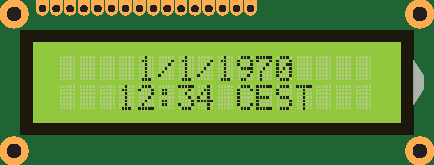
\includegraphics[width=0.6\columnwidth]{images/screen5}
  \caption{Pantalla 5 del módulo interior -- fecha y hora}
  \label{fig:screen5}
\end{figure}

\item[Pantalla 5: fecha y hora] --- Esta pantalla muestra la fecha y hora según la zona horaria que se ha establecido en las opciones de configuración (de nuevo, ver sección~\ref{sec:params-interior}). Dadas las características del hardware del \CMS (que no dispone de reloj interno), la fecha y la hora se obtienen de internet. La primera línea muestra la fecha, mientras que la segunda muestra la hora y la zona horaria, por ejemplo, CEST (\textit{Central European Summer Time} u hora de verano de Europa central), CET (\textit{Central European Time} u hora de invierno de Europa central),~\etc

\end{descriptioncompact}


\subsection{Avisos y alarmas sonoras}
\label{sec:alarmas}

Además de los testigos luminosos, el \CMS puede lanzar avisos y alarmas sonoras para alertar de los eventos críticos que requiren de una acción in\-me\-diata del usuario.

\tipbegin{Modo silencio permanente}
Es posible desactivar todas las alarmas sonoras de forma permanente colocando el interruptor de la alarma sonora \circled{I8} en la posición \off.
\tipend

\tipbegin{Silencio automático}
Además del modo de silencio permanente, el \CMS puede silenciarse automáticamente durante una determinada franja horaria, por ejemplo, para evitar avisos sonoros durante la noche. Vea la sección~\ref{sec:params-interior} (\textit{\nameref{sec:params-interior}}) para más información.
\tipend

\tipbegin{Comprobación de estado de las alarmas sonoras}
En caso de duda, es posible comprobar si el \CMS se encuentra en modo de silencio permanente pulsando el botón de reinicio \circled{I5} ---o desconectando momentáneamente la alimentación USB \circled{I6}--- del \MIE. Si el modo de silencio permanente está \textbf{activado}, el \CMS no emitirá ningún sonido. Si el modo de silencio permanente está \textbf{desactivado}, el \CMS emitirá tres pitidos cortos al iniciarse. \textbf{Los tres pitidos se emitirán incluso en el periodo de silencio automático.}
\tipend


Los avisos y alarmas que emite el \CMS son:

\begin{descriptioncompact}

\item[Aviso de batería baja] --- Cuando la tensión proporcionada por la batería del \MEE está por debajo del umbral configurado (véase \emph{Umbral de batería baja} en la sección~\ref{sec:params-interior}), el \MIE lo notifica regularmente emitiendo un breve pitido agudo en todas las horas en punto ---o en la primera sincronización cuando el \CMS acaba de conectarse--- hasta que las baterías son reemplazadas.

Recuerde que cuando el \ME notifica un valor por debajo del \emph{Umbral de batería baja}, el testigo de conexión \circled{I4} (\circlefilled{green}) permanece encendido de forma intermitente.


\item[Alarma de depósito lleno] --- Cuando el \MEE notifica que el depósito se ha llenado, el \MIE emite breves pitidos graves de forma continua durante 60 segundos (o hasta que se pulsa el botón multifución \circled{I8}).
La secuencia de pitidos de 60 segundos de duración se repite cada varios minutos (según el \emph{Tiempo de espera entre mensajes}, véase la sección~\ref{sec:params-exterior}) mientras el depósito permanece lleno.

Cuando el aviso de depósito lleno se dispara, el menú de información del \MIE se bloquea, la pantalla LCD \circled{I1} muestra el mensaje \emph{!!! ALERTA !!! / DEPO\-SITO LLENO} (ver figura~\ref{fig:screen-deposit-full}), y el testigo de fallo \circled{I2} (\circlefilled{red}) permanece encendido de forma intermitente hasta que se vacía el depósito. 

\begin{figure}
  \centering
  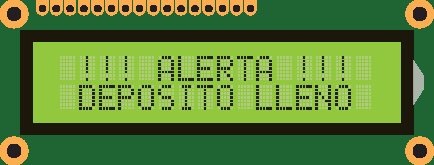
\includegraphics[width=0.6\columnwidth]{images/screen-deposit-full}
  \caption{Pantalla del módulo interior: depósito lleno}
  \label{fig:screen-deposit-full}
\end{figure}

\begin{figure}
  \centering
  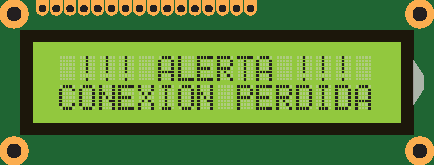
\includegraphics[width=0.6\columnwidth]{images/screen-conn-lost}
  \caption{Pantalla del módulo interior: conexión perdida}
  \label{fig:screen-conn-lost}
\end{figure}

\item[Alarma de conexión perdida] --- Cuando el \MIE no recibe ninguna información por parte del \MEE durante demasiado tiempo (véase \emph{Tiempo de espera máximo} en la sección~\ref{sec:params-interior}, \textit{\nameref{sec:params-interior}}), el \MIE emite un pitido agudo y un pitido grave ---emulando una sirena--- de forma continua hasta que la conexión con el \MEE se restaura o la alarma se silencia pulsando el botón multifunción \circled{I8}.   

Cuando el aviso de conexión perdida se dispara, el menú de información del \MIE se bloquea, la pantalla LCD \circled{I1} muestra el mensaje \emph{!!! ALERTA !!! / CONEXION PERDIDA} (véase figura~\ref{fig:screen-conn-lost}), y el testigo de fallo \circled{I2} (\circlefilled{red}) permanece encendido de forma fija hasta que se restaura la conexión entre los módulos interior y exterior. 



\attbegin{En caso de conexión perdida}
En caso de conexión perdida, revise el procedimiento detallado en la sección~\ref{sec:conn-perdida} (\textit{\nameref{sec:conn-perdida}}).
\attend

\end{descriptioncompact}


\cleardoublepage

